\chapter{La metodologia}
\label{chap:cap4}
\textbf{Francesco: non classifichi file audio...ma applicazioni Android attraverso file audio...}
In questo capitolo esporremo la metodologia utilizzata per la classificazione delle applicazioni Android, attraverso file audio. Nello specifico partiremo dai software e dai tipi di dati utilizzati per poi muoverci verso l'estrazione delle feature, la generazione dei dataset e la classificazione attraverso una particolare tecnica di machine learning chiamata multiple instance learning (MIL). 
\begin{figure}[h]
\centering
    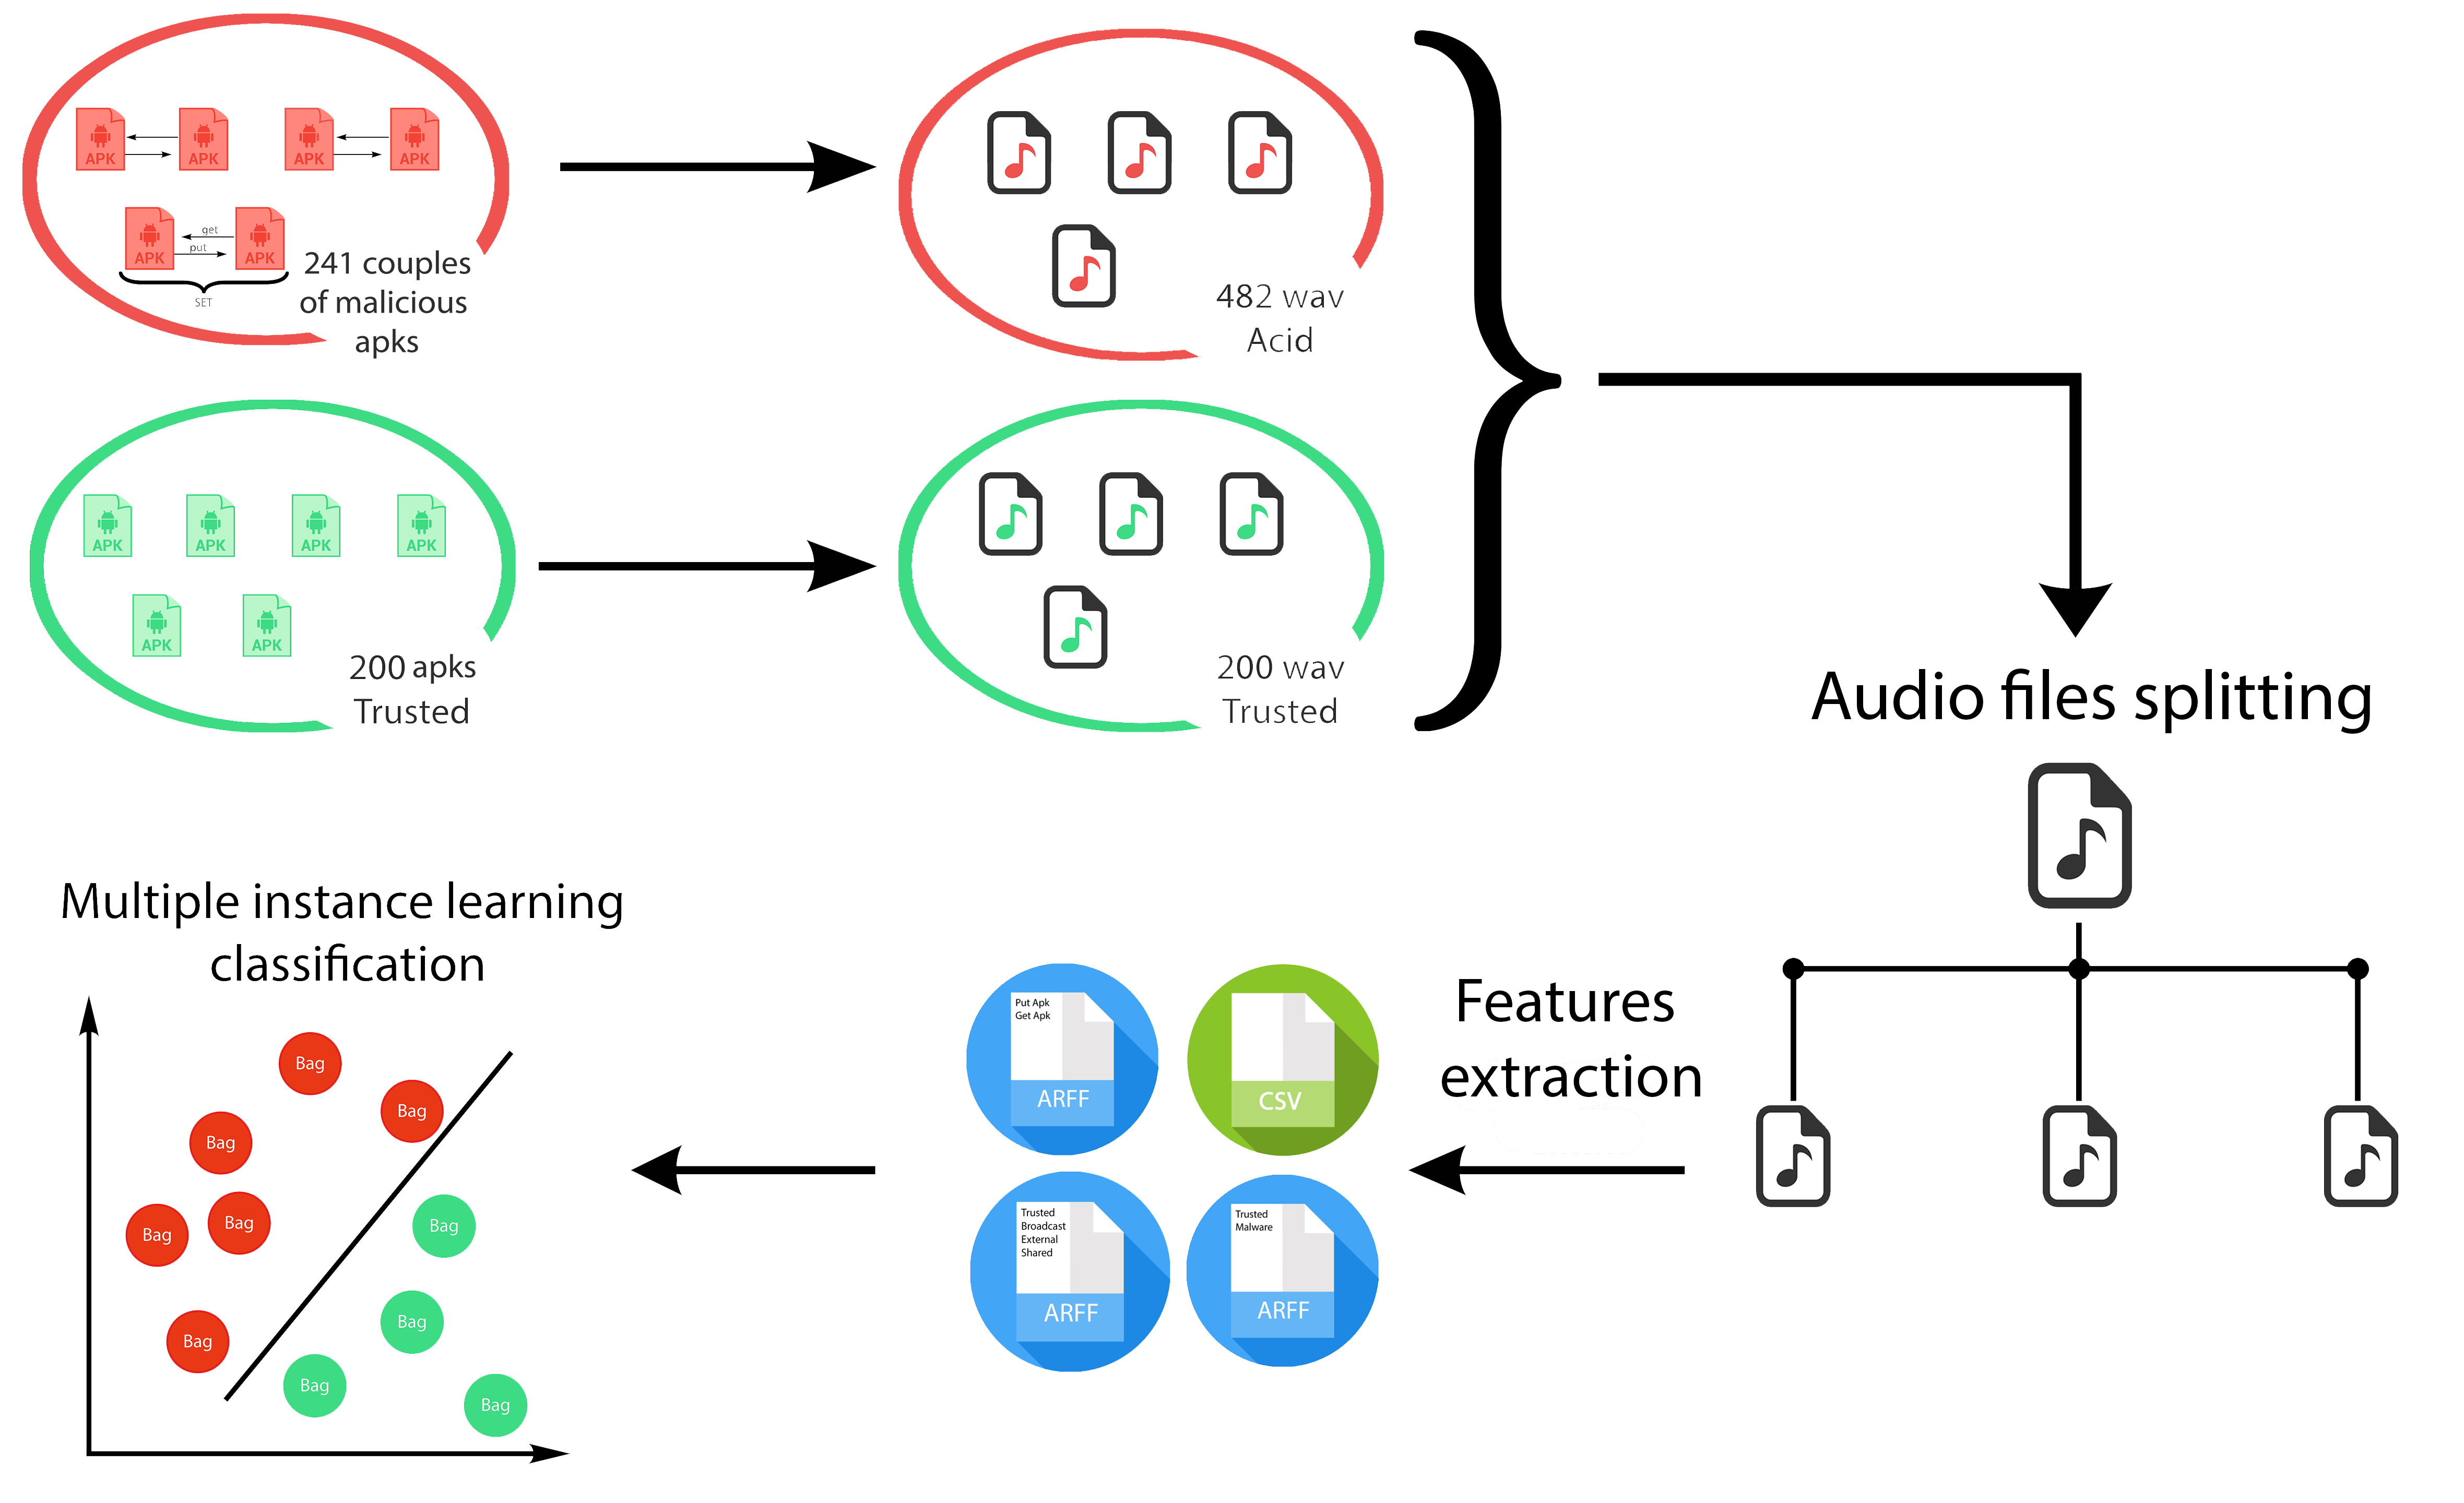
\includegraphics[width=0.9\linewidth]{imgs/capitolo4/engall.png} 
    \caption{Methodology of development  }
    \label{fig:all}
\end{figure}
\FloatBarrier
\section{I software e i dataset}
In questo paragrafo esporremo dapprima tutti i software utilizzati nell'analisi e una breve panoramica sulle caratteristiche principali dei dataset utilizzati.  
\subsection{WEKA}
\label{par:weka}
Acronimo di "Waikato Environment for Knowledge Analysis", è un software open source per il machine learning. Partendo da un dataset\footnote{Collezione di dati organizzati, la grandezza è data dal numero di righe.} è possibile applicarvi dei metodi di apprendimento automatico e di analizzarne il risultato è inoltre possibile attraverso l'utilizzo di questi metodi avere una previsione su nuovi set di dati. Per poter utilizzare gli algoritmi di classificazione del multiple instance learning bisogna importare i relativi package, attraverso il tool "Package Manager" già presente di default nella schermata iniziale di weka. Figura \ref{fig:mil pckg}.
\begin{figure}[h]
\centering
    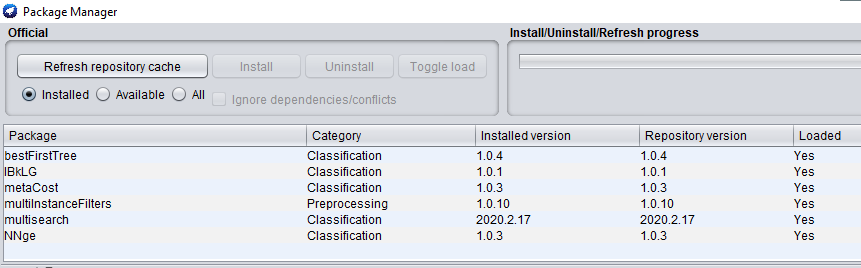
\includegraphics[width=0.9\linewidth]{imgs/capitolo4/packmil.png} 
    \caption{Input Mil package in weka}
    \label{fig:mil pckg}
\end{figure}
\FloatBarrier
Una particolarità di questo software è l'utilizzo di dataset .arff 


\subsection{dataset.csv e dataset.arff}
\label{par:dataset}
I dataset utilizzati nel progetto sono dataset con estensione \textbf{.csv - Comma Separated Values}, questo è un formato di file di testo in cui ogni riga rappresenta un record della tabella. Ogni colonna invece rappresenta dei valori associati ad ogni record. Le colonne sono separate da virgole, da qui il nome. In figura \ref{Fig:Datacsv} è possibile osservarne un esempio. 
\vspace{1em}
\newline
Il secondo tipo di dataset che abbiamo utilizzato sono file dati con estensione \textbf{.arff - Attribute Relationship File Format} come suggerisce il nome, questo formato di file organizza i dati seguendo una logica relazionale.
La formattazione del dataset utilizzato è stata realizzata in ottica di una classificazione attraverso algoritmi di multiple instance learning, dunque si è reso necessario dover organizzare i dati in bag. L'inizializzazione del file, per una classificazione MIL\footnote{Mil - Multiple instance learning} può essere suddiviso in cinque componenti\cite{wekaDoc}:  
\begin{enumerate}
        \item Nella prima va sempre definita la relazione che lega i dati attraverso l'attributo \textbf{@relation} ed un nome che descriva quello che vogliamo predire.  
        
        \item Successivamente andranno inseriti gli identificativi delle bag, ovvero utilizzando \textbf{@attribute bag\_id \{...\}} si vanno ad inserire nelle parentesi graffe la lista di tutti gli identificativi delle istanze della bag. Ogni identificativo va separato dall'altro tramite tramite l'utilizzo di una virgola. 
        
        \item Dopo si definiranno gli attributi della bag, per farlo si utilizza \textbf{@attribute bag relational} per definire l'inizio della bag ed \textbf{@end bag} per definire la fine della bag. All'interno, tra i due attributi, vanno specificati gli attributi che compongono le istanze di una bag, ovvero le caratteristiche dei dati. Per farlo si utilizza ancora una volta l'identificativo \textbf{@attribute nome\_caratteristica tipo\_caratteristica}. Il tipo di caratteristica può essere \textit{numeric} se il valore del dato è un numero intero, altrimenti \textit{real} se il tipo di attributo è un numero reale altrimenti. Se invece il tipo di attributo è una stringa scriveremo i valori ammissibili presenti tra parentesi graffe es. {\{yes, no\}} nel caso di un attributo booleano.
        
        \item A questo punto dobbiamo definire la classe che rappresenta una istanza. Per farlo inseriremo i valori tra parentesi graffe definendo l'attributo class come, \textbf{@attribute class \{calss1, class2\}}
        
        \item Infine a capo della key \textbf{@data} inseriremo il dataset correttamente formattato nel seguente modo: iesima bag\_id + ',' poi dovremmo definire tutte le istanze della bag. Una bag si definisca all'interno delle virgolette "...". Inseriremo all'interno tutte le istanze ognuna della quali sarà separata dal carattere speciale '$\backslash$n'. A loro volta ogni istanza è rappresentata dai diversi attributi, tanti quanti ne abbiamo definiti in precedenza, ogni attributo d'istanza è separato dall'altro tramite ','. Infine dopo la chiusura delle virgolette inseriamo la virgola e va definita la classe della bag. Ogni riga ha quindi la seguente formattazione:
        \\\footnotesize {
        bag\_id , " attr1Ist1, attr2Ist1, attr3Ist1 $\backslash$n attr1Ist2, attr2Ist2, attr3Ist2 $\backslash$n attr1Ist3, attr2Ist3, attr3Ist3 " , classe  }
    \end{enumerate}
\begin{figure}[h]
   \begin{minipage}{0.48\textwidth}
     \centering
     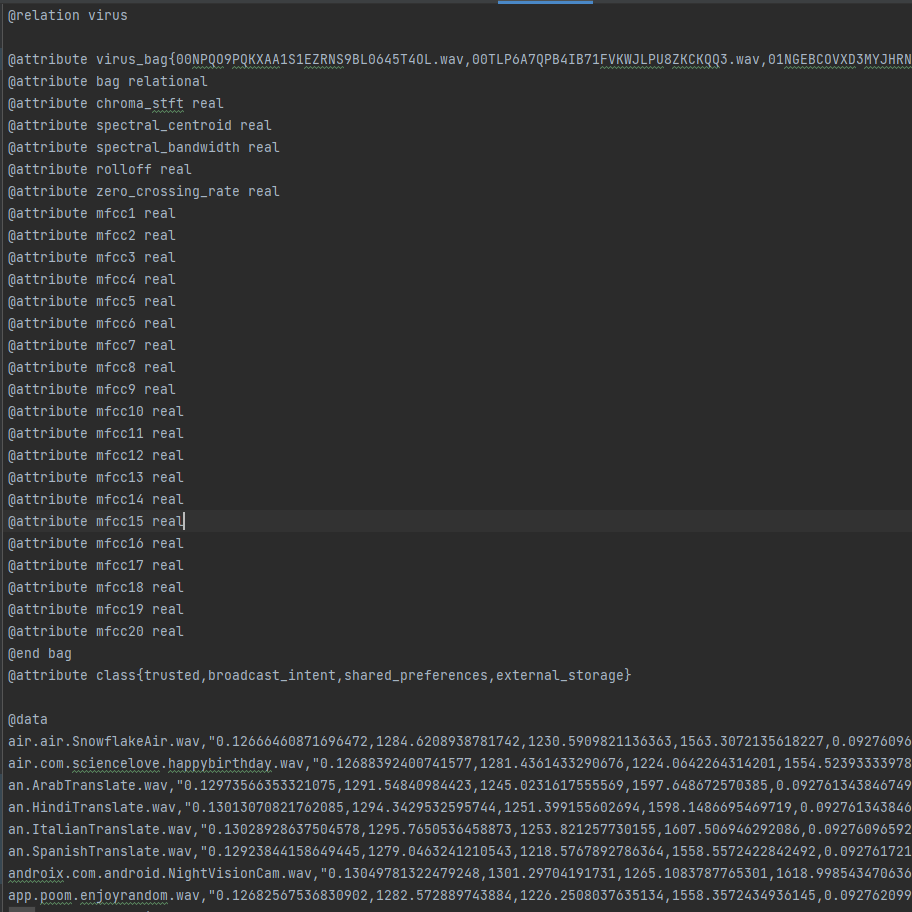
\includegraphics[width=0.85\linewidth]{imgs/capitolo4/ARFF.png}
     \caption{ARFF dataset for MIL}
     \label{Fig:Dataarff}
   \end{minipage}\hfill
   \begin{minipage}{0.48\textwidth}
     \centering
     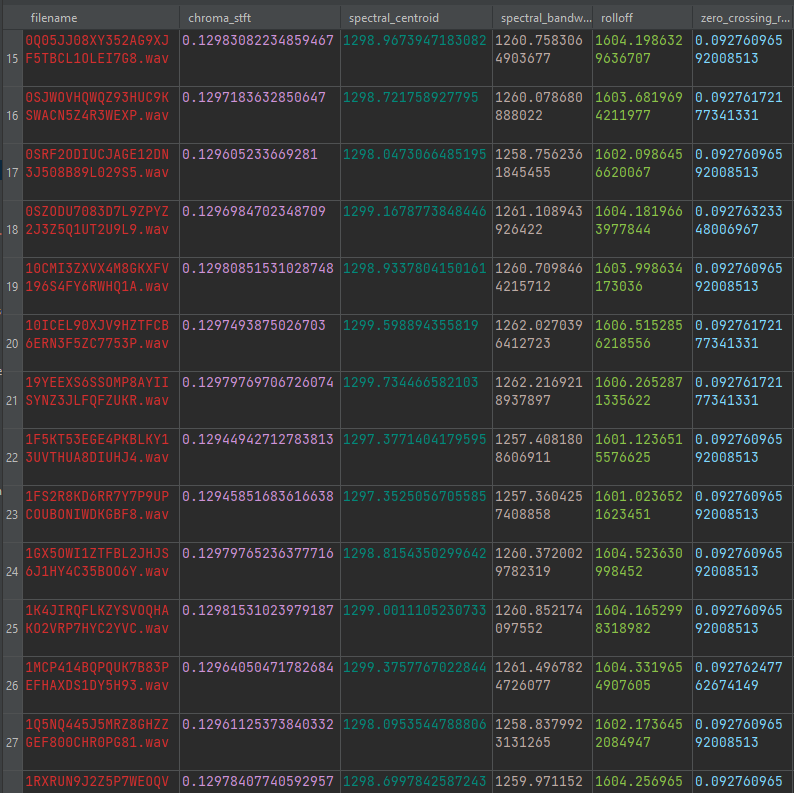
\includegraphics[width=0.85\linewidth]{imgs/capitolo4/csv.png}
     \caption{CSV file}
     \label{Fig:Datacsv}
   \end{minipage}
\end{figure}
\FloatBarrier 
\subsection{Dataset di applicativi android}
\label{par:datasetApk}
Siamo partiti da due dataset di applicazioni apk. Il primo conteneva un set di 200 applicazioni android non affette da malware che abbiamo definito come dataset "trusted", il secondo dataset invece conteneva 241 coppie di apk affette da malware abbiamo definito questo dataset come "Acid". Quest'ultimo dataset come detto comprendeva 241 set ognuno dei quali includeva due package APK. Nello specifico queste due applicazioni, affette da malware, comunicano tra loro attraverso lo scambio nascosto di informazioni e vengono quindi dette \textit{colludenti}. Di fatti una applicazione è di tipo "PUT" e l'altra è di tipo "GET". Per un totale di 482 applicazioni colludenti, si hanno 241 applicazioni di tipo "GET" e 241 di tipo "PUT".

\section{Elaborazione dei file audio}
In questo paragrafo descriveremo l'elaborazione dei file audio, ovvero la loro generazione/conversione e la successiva suddivisione.

\subsection{Generazione dei file audio}
\label{par:gen}
Lo script realizzato per la conversione di un applicativo android in un file audio, una volta inserito nella directory che contiene i due dataset di apk, va dapprima ad individuare tra i tutti i file che compongono un dataset i soli package .apk, successivamente va a decomprimere ogni pacchetto e ad estrarre da ognuno il file classes.dex. Questo file viene elaborato e  convertito in un file audio con estensione WAV. L'output è salvato in una cartella creata ad hoc per raccogliere tutti i file audio generati,  suddividendo i file audio generati da applicativi "trusted" da quelli di tipo "Acid", creando una directory di output differente a seconda del tipo. 

\subsection{Splitting dei file audio}
Il secondo script sviluppato chiede in input la durata dello split in secondi, la durata dev’essere maggiore di 0.
Controllando che non sia stata creata in precedenza, va ad inizializzare una cartella "Splitted" tramite una funzione “createNewDirectory” [Listing:\ref{lst:newDir}].
\begin{lstlisting}[language=Python, caption=Create new directory function, label = lst:newDir]
def createNewDirectory(path=os.getcwd(), nameNewDirectory=""):
    pathNewDirectory = path + "\\" + nameNewDirectory
    if not os.path.exists(pathNewDirectory):
        try:
            os.mkdir(pathNewDirectory)
            print("Directory created successfully")
            return pathNewDirectory
        except OSError as error:
            print("Directory can not be created")
    else:
        return pathNewDirectory
\end{lstlisting}

Proseguendo va ad iterare su tutti i file audio WAV presenti nelle cartelle "trusted" ed "Acid" generate precedentemente dalla conversione delle applicazioni. [Listing:\ref{lst:audioOrig}]

\begin{lstlisting}[language=Python, caption=Iteration over whole audios, label = lst:audioOrig]
for wav_file in os.listdir(unsplit_audio_folder):
    if wav_file.endswith(".wav"):
        wavSplittedDirectory = createNewDirectory(Path_SubDirectory, str(wav_file))
        pathToOriginalWav = unsplit_audio_folder + "\\" + str(wav_file) 
        splittingWav(pathToOriginalWav, wavSplittedDirectory)
\end{lstlisting}


Per ogni file WAV trovato si va a creare uan cartella in "\textit{Splitted\textbackslash nameFileAudio}" dove il nome della directory è dato dal file .wav da splittare. Questa nuova cartella sarà poi popolata con i file splittati risultanti. In questo modo ogni file .wav avrà una sua directory che conterrà gli split di output.\\
Lo split avviene in una funzione “splittingWav” che va a calcolare il numero degli split in cui suddividere il file audio originale. Il calcolo avviene tramite una divisione per eccesso, in questo modo si includono anche suddivisioni più piccole del numero dato in input. Successivamente iterando sugli intervalli crea la suddivisione, partendo di volta in volta dal file della durata intera, come si può osservare in figura \ref{fig:split1} e \ref{fig:split2}.
\begin{figure}[h]
   \begin{minipage}{0.48\textwidth}
     \centering
     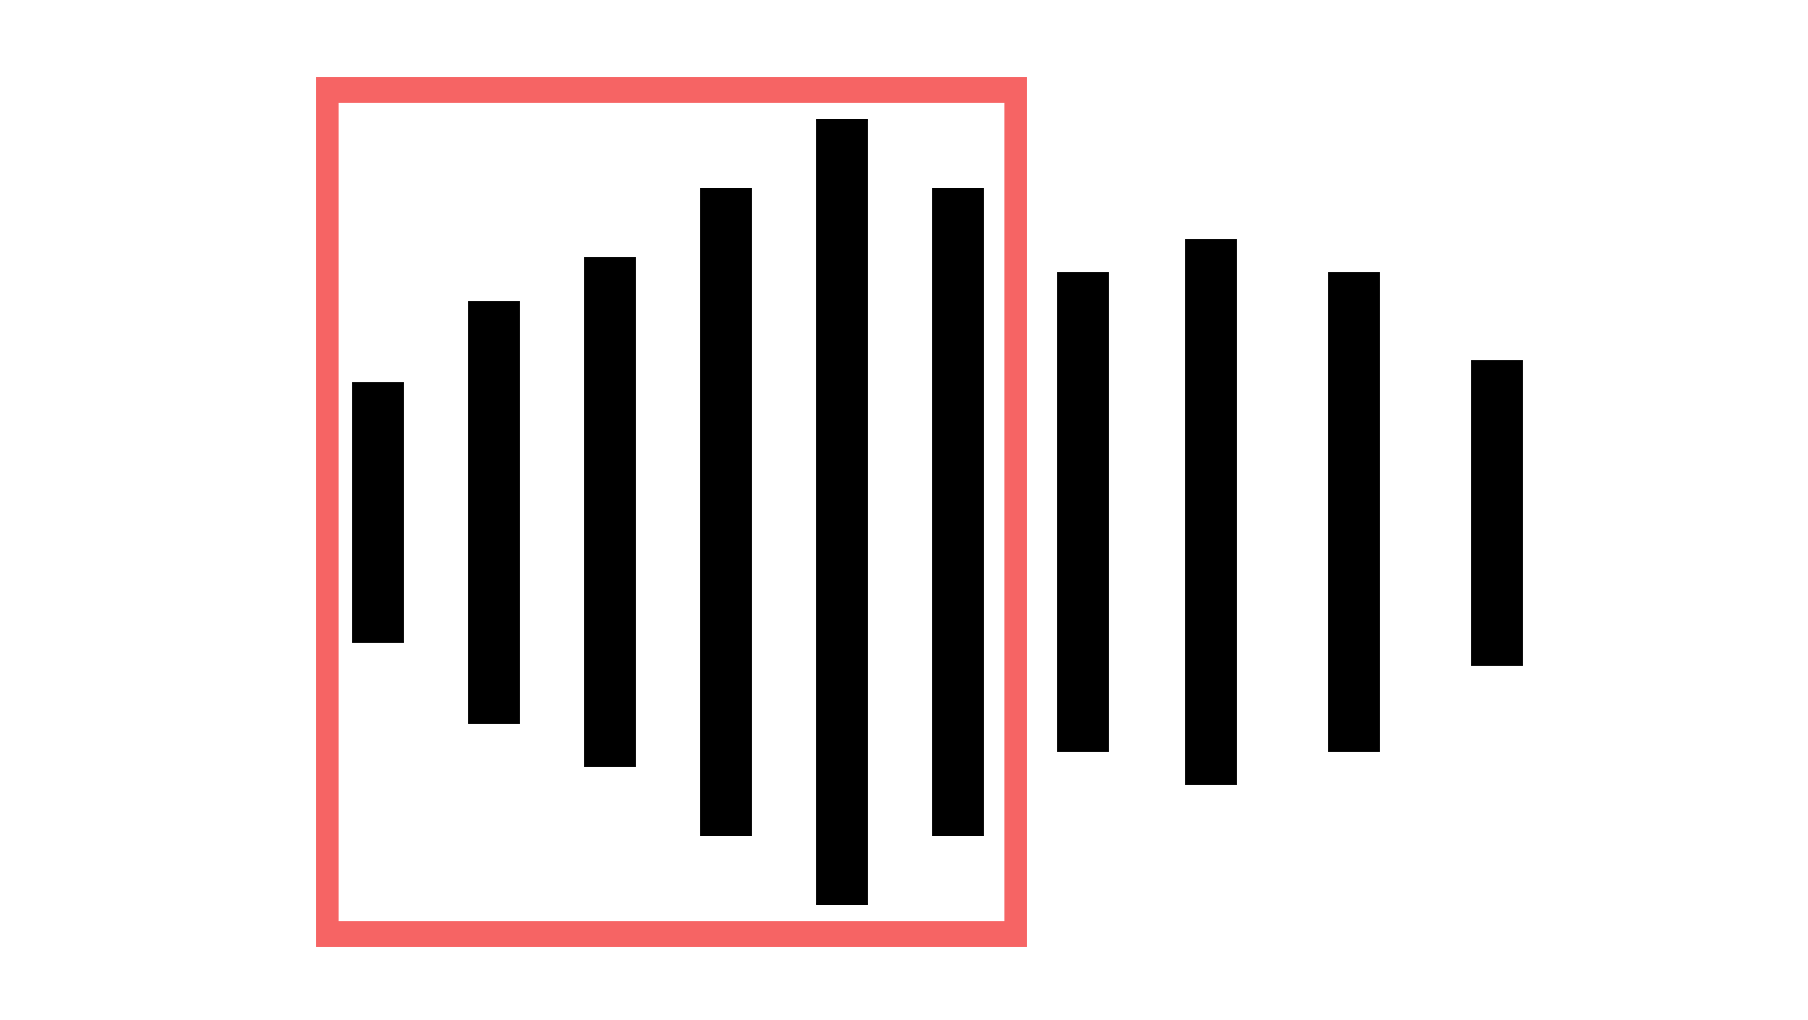
\includegraphics[width=0.85\linewidth]{imgs/capitolo4/suddivisione.png}
     \caption{first split}
         \label{fig:split2}
   \end{minipage}\hfill
   \begin{minipage}{0.48\textwidth}
     \centering
     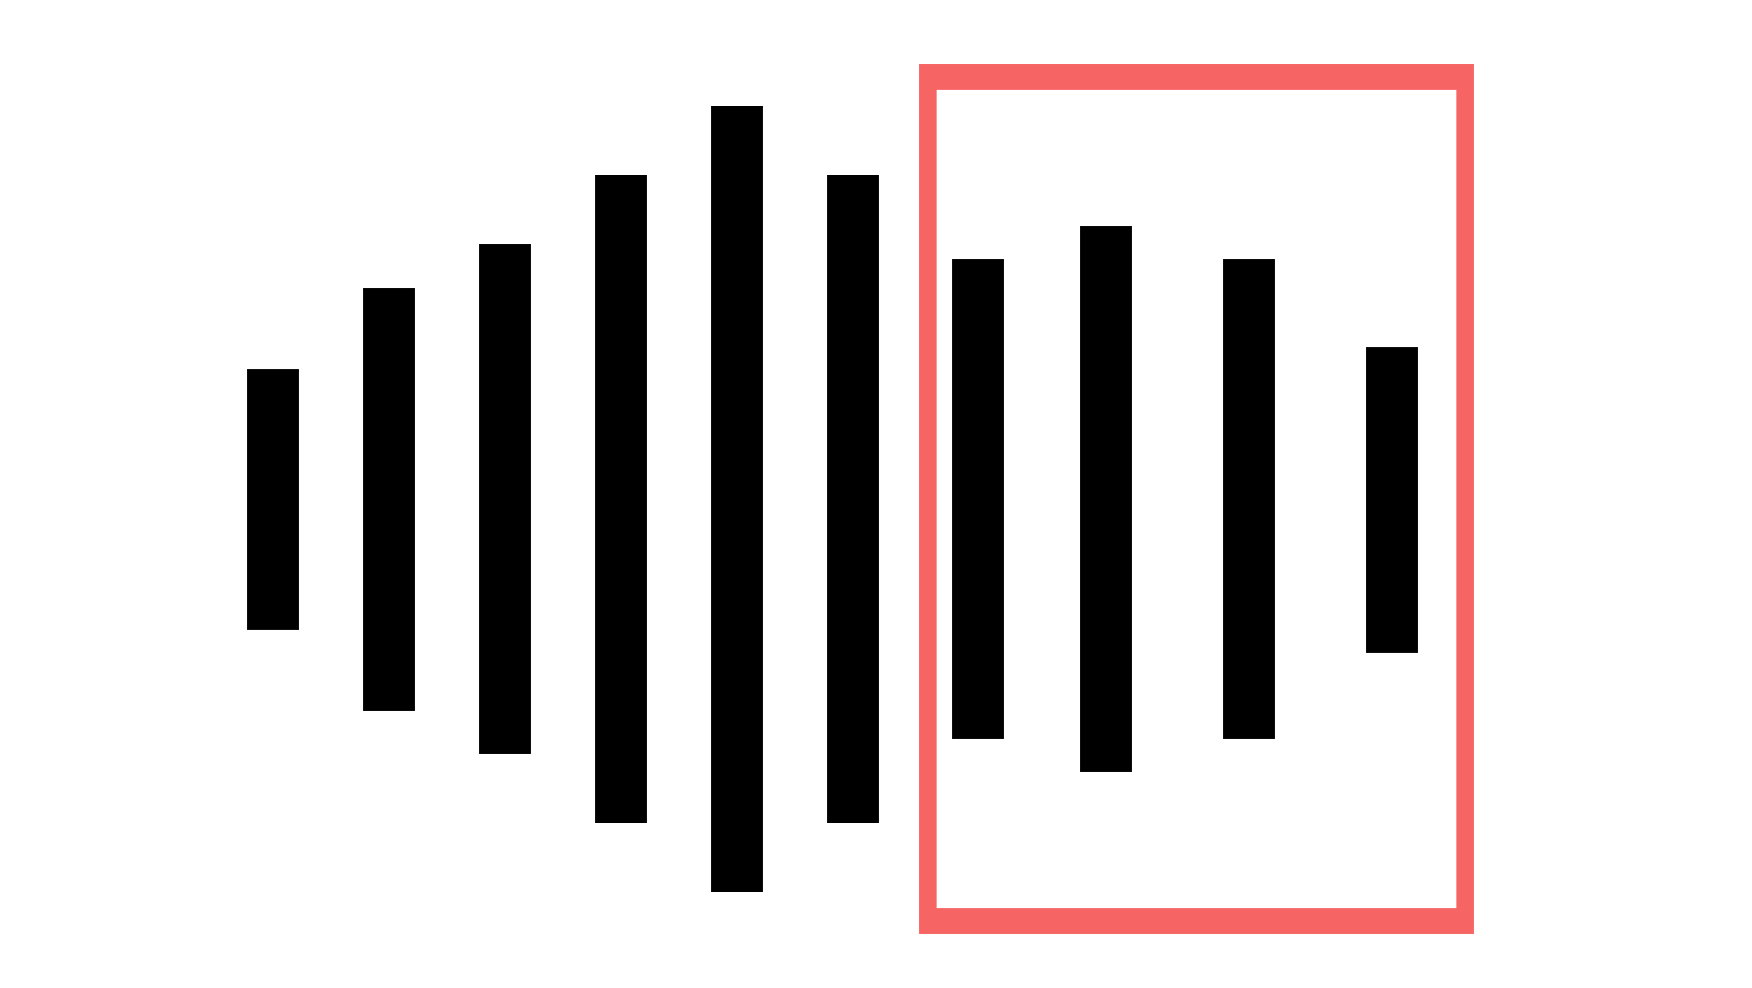
\includegraphics[width=0.85\linewidth]{imgs/capitolo4/suddivisione2.png}
     \caption{second split}
     \label{fig:split1}
   \end{minipage}
   
\end{figure}
\FloatBarrier 
La libreria utilizzata per effettuare lo splitting dei dati è \href{https://github.com/jiaaro/pydub#installation}{"pydub"}\cite{pydub}. Nel codice le variabili @t\_start e @t\_stop rappresentano per ogni iterata il punto d'inizio e quello di fine dell'i-esimo split del file. Il nome dei file splittati corrispondono all’intervallo dell’i-esimo split (in millisecondi). 

\begin{lstlisting}[language=Python, caption=Splitting wav function, label = lst:splitFun]
def splittingWav(pathToOriginalWav, pathToSplittedWav):
    #Load
    originalAudio = AudioSegment.from_wav(pathToOriginalWav)
    numberOfSplit = math.ceil(originalAudio.duration_seconds / splittingduration)
    t_start = 0
    
    for i in range(numberOfSplit):
        t_stop = (t_start + (splittingduration * 1000))  
        splittedAudio = originalAudio[t_start:t_stop]
        splittedAudio.export(out_f=pathToSplittedWav + "\\" + str(t_start) + " - " + str(t_stop) + '.wav',format="wav")         
        t_start = t_stop
\end{lstlisting}

\section{Estrazione delle features}
\label{par:feat}
Al fine di poter effettuare una classificazione abbiamo bisogno di attributi che possano rappresentare un dato oggetto, nel nostro caso un audio digitale. Il suono in natura è un segnale continuo, dunque per essere memorizzato dev'essere campionato ottenendo in questo modo un segnale digitale rappresentato da valori numerici che vadano ad approssimare il più possibile la forma dell'onda. Ogni campione è formato da un dato numero di bit e viene prelevato con ritmo constante dal suono. Una frequenza di campionamento rappresenta il numero di campioni prelevati in un secondo ed è un numero che di solito oscilla tra gli 8000 ed i 44100 samples al secondo.
\\\\ 
Lo scopo dello script per l'estrazione delle feature è quello di andare a generare tre dataset: 
\begin{itemize}
    \item \textit{data.arff}: Un dataset .arff, che verrà utilizzato per la calssificazione, che conterrà tutte le feature estratte per ogni singolo audio splittato, organizzando le istanze per la classificazione tramite multiple instance learning come descritto nel paragrafo [\ref{par:dataset}]. In questo dataset l'attributo \textbf{class} assume uno dei valori, "trusted", "broadcast\_intent", "shared\_preferences" o "external\_storage". Per estrarre questi attributi si va a leggere contenuto del file di accompagnamento "desctiption.txt" all'interno di ogni set Acid. Nel caso si sta analizzando un file audio generato da un apk trusted l'attributo verrà semplicemente impostato come "trusted".
    \begin{lstlisting}[language=Python, caption=Get android resources, label = lst:getREs]
     with open(f'{acidDatasetFolder}\\{setFold}\\{"description.txt"}', 'r') as reader:
                                    malwareType = reader.read().split(":")[1]
                                    classe = malwareType
    \end{lstlisting}
    \item \textit{dataBinary.arff}: Questo dataset, utilizzato per la calssificazione, conterrà tutte le feature estratte, ancora una volta, per ogni singolo audio splittato, organizzando i dati in bag. La differenza sta nell'andare ad inserire come attributi della \textbf{class} solamente i valori, "trusted", "malware".
    \item \textit{data.csv}: Il dataset.csv comprenderà solamente le applicazioni provenienti dal dataset "Acid". Le tre colonne che compongono la tabella sono riempite nel seguente modo. Nella prima andranno i nome delle bag\_id, nella seconda, le features delle varie istanze della bag ed infine nella terza colonna l'attributo \textbf{class} che può assume uno dei valori, "trusted", "broadcast\_intent", "shared\_preferences" o "external\_storage". Questo dataset sarà utilizzato per generare un quarto dataset "dataGetPut.arff" come vedremo nel paragrafo \ref{subsub:quartodata}. 
\end{itemize}

Lo script realizzato per estrarre le features, inizializzerà da prima i file dataset di cui sopra, che saranno poi utilizzati per organizzare le features. Lo script provvederà ad iterare nelle cartelle "Acid\_Splitted" e "Trusted\_Splitted" il cui contenuto sono le subdirectory con gli audio splittati generati dallo script precedente [\ref{par:gen}]. Per ogni audio contenuto nelle subdirectory si procede quindi all'estrazione delle features con l'ausilio della libreria "librosa"\cite{libosa}.
Attraverso:
\begin{lstlisting}[language=Python]
 y, sr = librosa.load(splittedAudioPath, mono=True, duration=30)
\end{lstlisting}
Si va a caricare il file audio in formato mono. la variabile "y" rappresenta la serie temporale dell'audio, dunque y[t] corrisponde all'ampiezza della forma dell'onda al campione t-esimo. Mentre la variabile "sr" rappresenta la frequenza di campionamento di "y". 
Successivamente attraverso le istruzioni: 
\begin{lstlisting}[language=Python]
            chroma_stft = librosa.feature.chroma_stft(y=y, sr=sr)
            spec_cent = librosa.feature.spectral_centroid(y=y, sr=sr)
            spec_bw = librosa.feature.spectral_bandwidth(y=y, sr=sr)
            rolloff = librosa.feature.spectral_rolloff(y=y, sr=sr)
            zcr = librosa.feature.zero_crossing_rate(y)
            mfcc = librosa.feature.mfcc(y=y, sr=sr)
\end{lstlisting}
\begin{itemize}
\item chroma\_stft: Calcola a partire dall'onda un cromogramma e ritorna un valore normalizzato di ogni frame. 
\item spectral\_centroid: Calcola il centroide spettrale. L'intensità di un suono in funzione del tempo e della frequenza può essere rappresentato graficamente da uno spettrogramma. Ogni fotogramma di uno spettrogramma viene normalizzato e ne viene estratta la media(centroide).
\item spectral\_bandwidth: Calcola la frequenza della larghezza di banda di ogni frame.
\item spectral\_rolloff: Calcola per ogni frame la frequenza di rolloff.
\item zero\_crossing\_rate: Calcola i passaggi per lo zero in una serie temporale.
\item mfcc: Genera una sequenza di coefficienti cefalici mfcc da una serie temporale.
\end{itemize}
Per ognuno di questi valori è stata estratta la media, ed il risultato inserito nella stringa che poi comporrà una riga del dataset. All'interno del codice sono inseriti diversi controlli per far si che la stringa rispetti la formattazione dei file di tipo ARFF. Infine la stringa, composta dal nome dell'audio (integro), dalle feature di tutti i singoli file audio (splittati) e dalla classe d'appartenenza, viene scritta in una nuova riga del file dataset corrispondente. 

\begin{lstlisting}[language=Python, caption=Arff formatting string, label = lst:splitFun]
                .............
            if (featureOfBag == 1):
                featureOfBag += 1
                to_append_arff = f'{audioTitle}{".wav"}{","}\"{np.mean(chroma_stft)}{","}{np.mean(spec_cent)}{","}{np.mean(spec_bw)}{","}{np.mean(rolloff)}{","}{np.mean(zcr)}{","}'
            else:
                to_append_arff += f'\\n{np.mean(chroma_stft)}{","}{np.mean(spec_cent)}{","}{np.mean(spec_bw)}{","}{np.mean(rolloff)}{","}{np.mean(zcr)}{","}'

            indexMfcc = 1
            for e in mfcc:
                if (indexMfcc == len(mfcc)): 
                    to_append_arff += f'{np.mean(e)}' 
                    to_append += f' {np.mean(e)}'
                else:
                    to_append_arff += f'{np.mean(e)}{","}' 
                    to_append += f' {np.mean(e)}{","}'
                indexMfcc += 1
            if splittedAudio != latestSplitter:
                to_append += "\\n"
                
                .............
                
            fileArff = open('results\\data.arff', 'a', newline='')
            fileArff.writelines(to_append_arff)
            fileArff.close()
\end{lstlisting}

Ogni dataset così generato è composto da 682 istanze che individuano le varie bag, con annesse istanze. Ogni bag corrisponde ad una applicazione. 

\subsubsection{Creazione del quarto dataset}
\label{subsub:quartodata}
Per generare il quarto dataset \textbf{dataGetPut.arff} abbiamo realizzato uno script che lavora su un dataset "smistamento.csv" contenente lo smistamento delle applicazioni. Ovvero in questo dataset sono elencati i nomi di ogni applicativo appartenete al dataset "Acid" e per ognuno e specificato se l'applicativo è di tipo "PUT" o "GET".  
\\Lo script quindi va a creare un nuovo file ARFF in cui verranno inserite le feature \textit{dataGetPut.arff}. Questo dataset sarà utilizzato per la classificazione. Di seguito dato in input il dataset "data.csv", creato attraverso lo script precedente [\ref{par:feat}], va a controllare per ogni istanza del dataset (data.csv) il tipo di classe di appartenenza nel secondo dataset (smistamento.csv) attraverso la ricerca di un uguaglianza del nome dell'applicativo. Infine va a scrivere nel datasetGetPut.arff creato le istanze, le features e la tipologia rilevata. 

\begin{lstlisting}[language=Python, caption=Application Get or Put control, label = lst:splitFun]
    for index, row in dataset_csv.iterrows():  
    typeWav = row[2]  
    nameWav = row[0]
    if typeWav == "trusted":
        continue
    else:
        type = str(getTypeOfApp(str(row[0]).split(".")[0])).replace(" ", "_")
        stringa = f'{nameWav}{","}\"{row[1]}\"{","}{type}\n'

        fileArff = open("results\\dataGetPut.arff", 'a', newline='')
        fileArff.writelines(stringa)
        fileArff.close()
\end{lstlisting}

\section{Il multiple instance learning}
In questo paragrafo faremo una breve panoramica sul \hyperref[subsub:mil]{multiple instance learning} prima però descriveremo  cos'è il  \hyperref[subsub:ml]{machine learning}. 
\subsubsection{Machine learning}
\label{subsub:ml}
Il machine learning è quella branca dell'intelligenza artificiale che si occupa di individuare schemi nei dati al fine di addestrare dei modelli per eseguire poi delle previsioni attraverso l'utilizzo di nuovi dati. I dati sono proprio il punto centrale di questa tecnologia, in quanto proprio il progressivo aumento di disponibilità degli stessi ha reso necessario lo sviluppo di algoritmi che fossero in grado di catturarne la conoscenza. I tipi di machine learning sono tre: 
\begin{enumerate}
    \item \textbf{Apprendimento supervisionato}: Questa tipologia si basa sull'addestramento di un modello, all'algoritmo viene dato in input il dataset da analizzare che comprende l'output atteso. I compiti possono dividersi in due sottocategorie, classificazione e regressione. 
    \begin{itemize}
        \item \textit{Classificazione}: L'obiettivo è, sulla base di osservazioni svolte in precedenza, di andare ad effettuare una predizione delle label di classi di nuove istanze. Le label sono un particolare valore, discreto, che rappresenta in qualche modo un gruppo di dati. Dunque il ruolo svolto dalla classificazione è quello di discriminare l'appartenenza di un set di dati ad una delle classi. A sua volta la classificazione può essere suddivisa in altre sottocategorie. Nel caso in cui le classi su cui effettuare una predizione è composta da due label, si dice che che stiamo effettuando una \textit{classificazione binaria}, altrimenti se le classi sono più di due ci troviamo di fronte ad una \textit{classificazione multiclasse}. 
        
        \item \textit{Regressione}: In questo caso sia l'input che l'output sono continui, di fatti dato in input un dataset, l'output sarà dato da un valore continuo. Ad esempio attraverso la regressione lineare data una variabile predittiva x ed una variabile risposta y, si va a calcolare la retta che va a minimizzare la distanza fra i punti e la retta\cite{pyML}.
    \end{itemize}
    \item \textbf{Apprendimento non supervisionato}: In questa categoria non sono note le classi del training set, la struttura dei dati può essere ignota, per l'estrazione delle informazioni dunque non si utilizza una variabile nota ne una funziona di ricompensa come vedremo nella prossima categoria. Un esempio è il \textit{clustering} in cui si vanno a ricercare dei sottogruppi che individuino relazioni tra i dati. 
    \item \textbf{Apprendimento con rinforzo}: In questa categoria, l'algoritmo di apprendimento sviluppa un sistema che migliori le prestazioni andando ad imparare dagli errori che ha effettuato in precedenza. Quindi il focus è di andare a massimizzare la ricompensa attraverso un approccio di tipo esplorativo. 
    
\end{enumerate}
Come si è potuto notare tutti gli approcci necessitano di un "ingrediente fondamentale" i dati. Uno dei passi primari è il pre-procssing dei dati come ad esempio la normalizzazione. 
Un ulteriore passaggio che va effettuato sul dataset, per la maggior parte degli algoritmi è la suddivisone di quest'ultimo in un \textit{training set} ed un \textit{test set}. Il primo viene utilizzato per la fase di addestramento del modello predittivo, il secondo per valutare la capacità di quanto il modello sia in grado di effettuare una predizione utilizzando nuovi dati, viene detto testing. 

\subsubsection{Multiple instance learning}
\label{subsub:mil}
Il Multiple instance learning rientra nell'apprendimento supervisionato. L'utilizzo di questa metodologia ha come caratteristica principale quella che l'organizzazione delle istanze avviene tramite particolari set che vengono chiamati \textit{bag}. Ad ognuna di queste bag viene associata una label, dunque un'etichetta riguarda tutte le istanze della bag\cite{enwiki:972908596}. Dunque ad un algoritmo di apprendimento automatico vengono date in input più bags, ognuna delle quali è composta da più istanze. 
L'obiettivo del MIL\footnote{Abbreviazione di multiple instance learning} è quello di prevedere la label di nuove bag non utilizzate nella fase di addestramento del modello. Lo sviluppo di questa metodologia si sta ampliando in quanto sono aumentati i dati disponibili e classificarli singolarmente, come avviene in un problema di classificazione standard richiede uno sforzo maggiore. Attraverso il MIL si allevia questo onere\cite{Carbonneau_2018} organizzando appunto i dati in bag contenenti le istanze ed assegnandoli un label. Un apprendimento tramite MIL consente di affrontare sia problemi di classificazione che di regressione. 
\\In questo lavoro le istanze che vanno a comporre una bag sono tutte le feature estratte da ogni audio splittato. Questo significa che ogni bag rappresenta una singola applicazione ed il suo contenuto è composto dall'insieme delle feature, ognuna estratta dal relativo file audio splittato dall'audio integro frutto della conversione dell'apk in .wav. La classe di una bag è invece data dal tipo di applicazione, se trusted o malware come specificato al paragrafo \ref{par:feat}

\section{K-fold validation}
\label{par:kfold}
La k-fold validation è una tecnica che va a dividere il dataset in k sezioni, utilizzando k-1 sezioni per il training e la k-ma sezione per il testing. La procedura viene poi ripetuta andando ad utilizzare una nuova sezione delle k calcolate precedentemente per il testing e le restanti k-1 per il training. Il tutto si ripete per k volte andando di volta in volta ad utilizzare un segmento differente per la fase di testing. Infine tra tutte le osservazioni si va a prendere la media. In WEKA l'algoritmo viene chiamato una k+1 esima volta sull'intero testi di dati\cite{kcross}. Questa tecnica è utile per dataset non molto popolati.  
\begin{figure}[h]
   \begin{minipage}{0.48\textwidth}
     \centering
     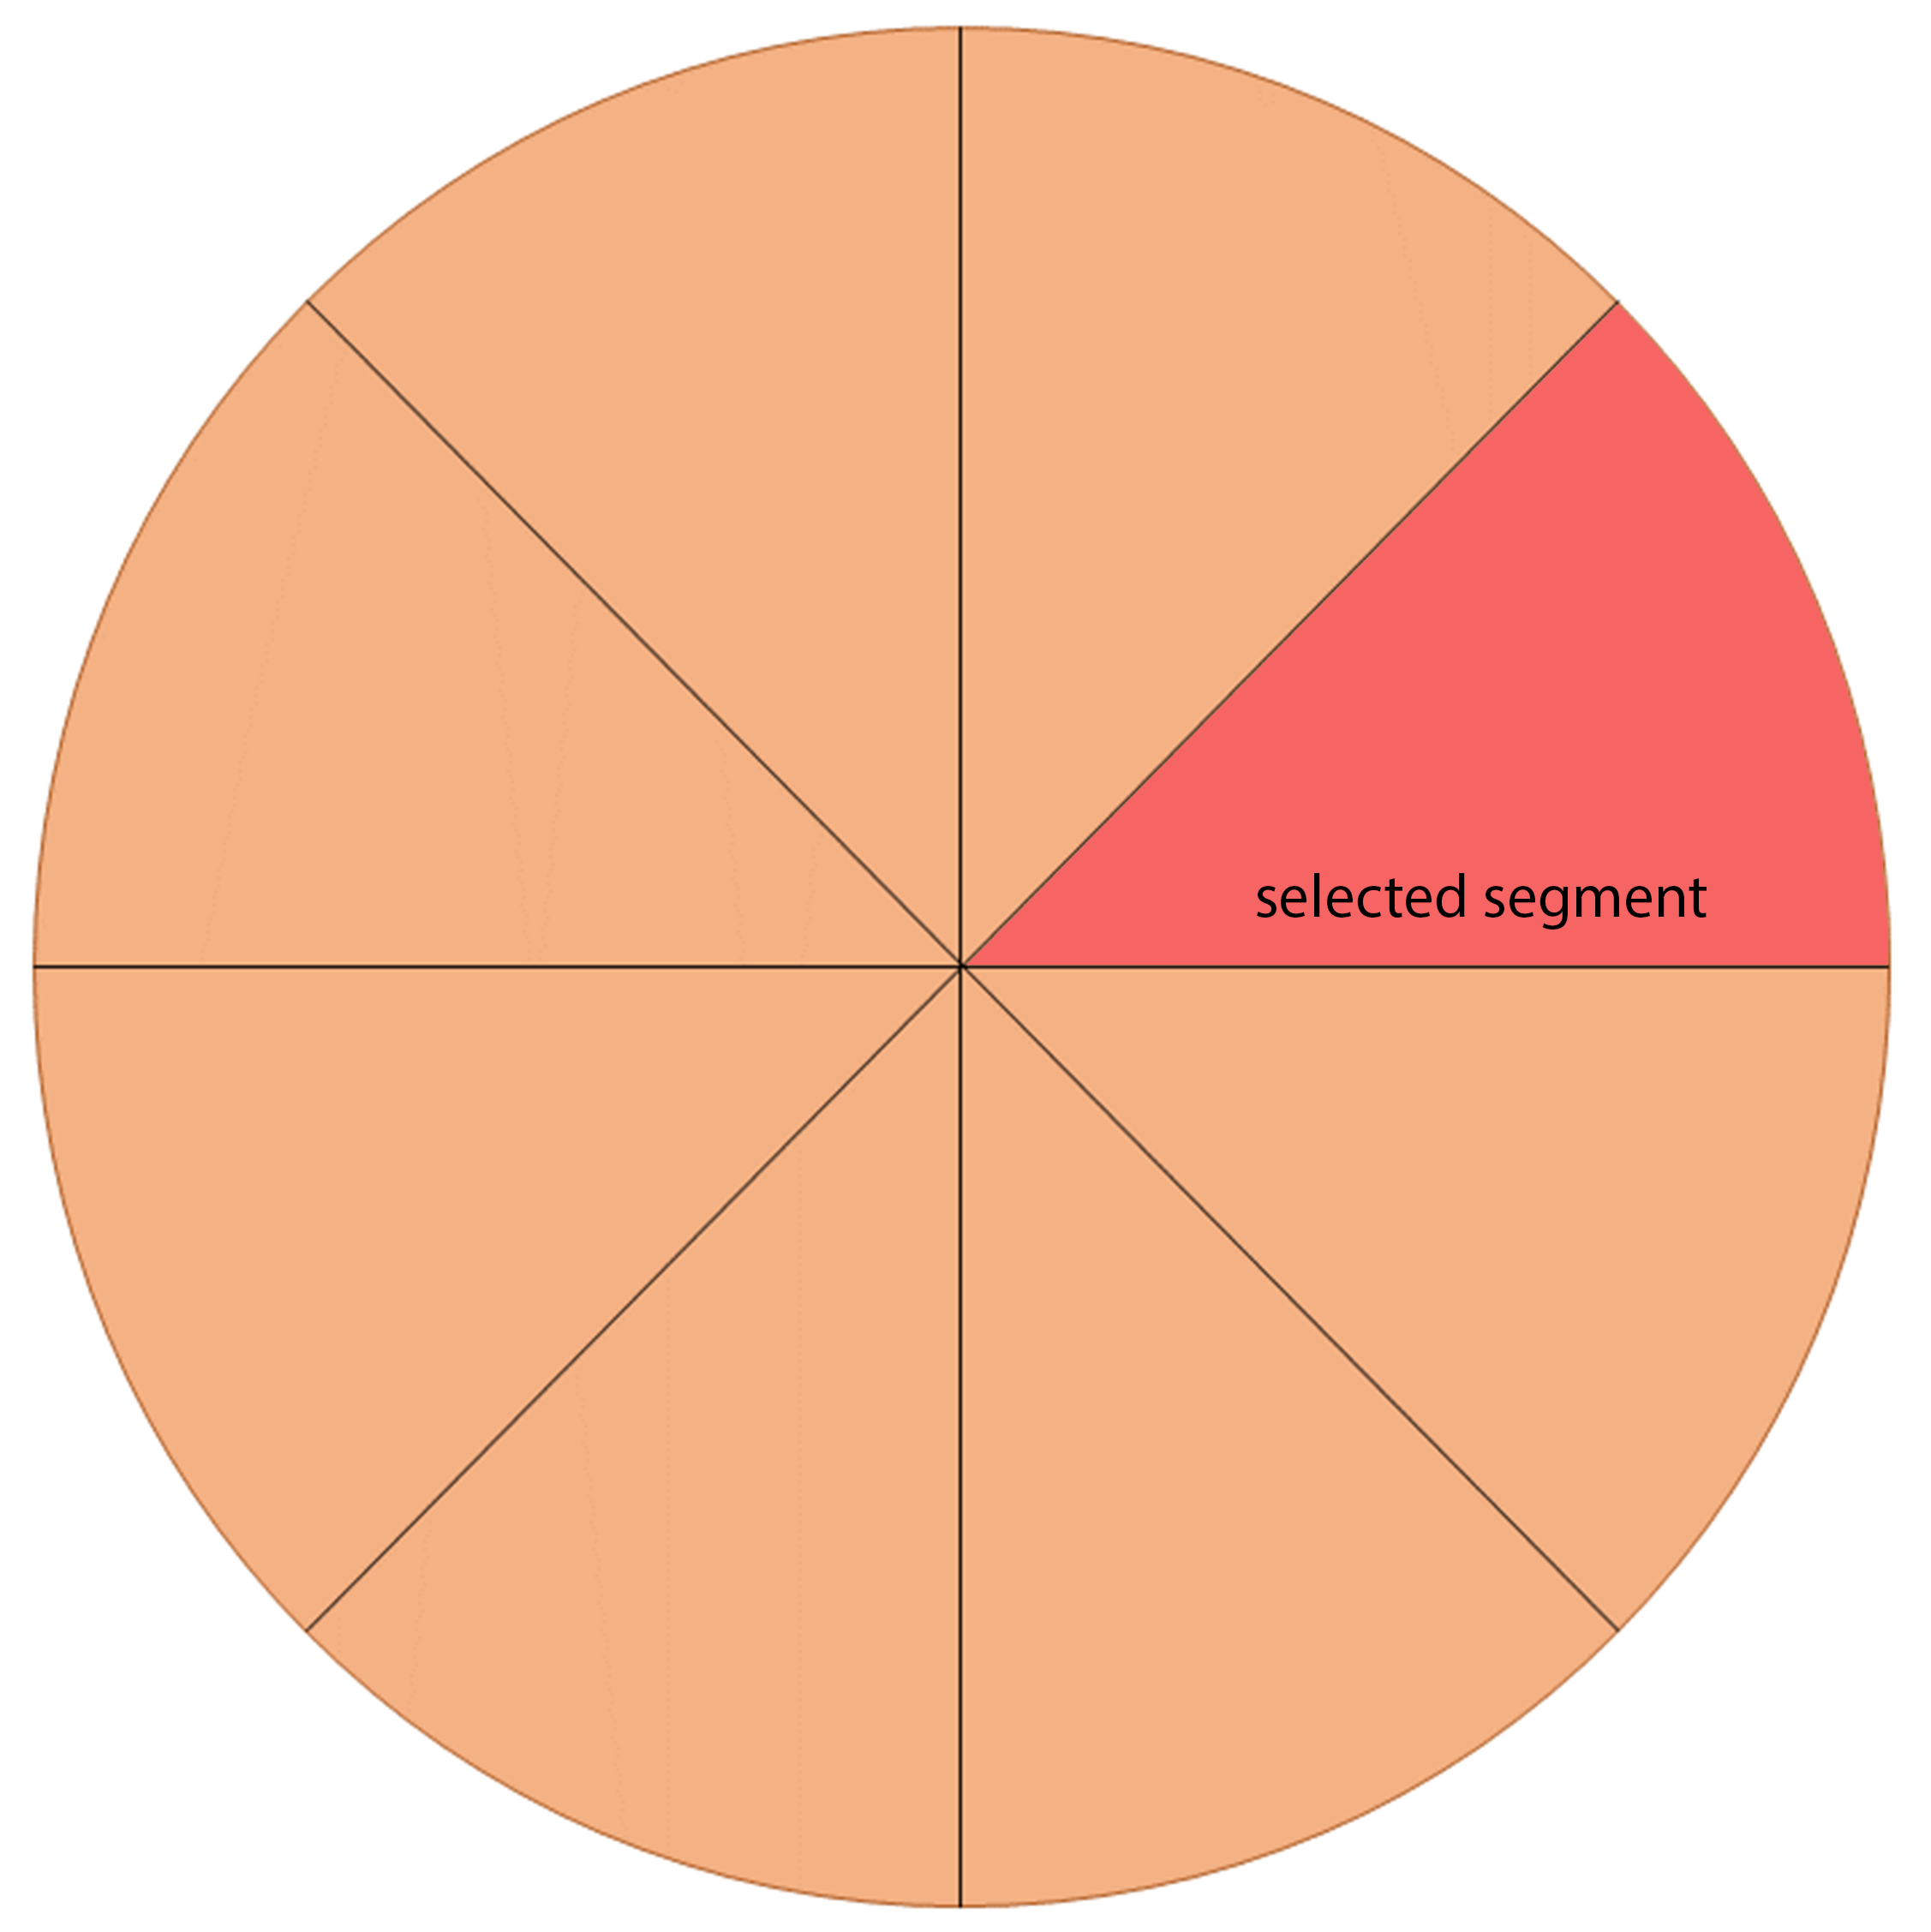
\includegraphics[width=0.60\linewidth]{imgs/capitolo4/kfold1.png}
     \caption{k th selected segment}
         \label{fig:cross}
   \end{minipage}\hfill
   \begin{minipage}{0.48\textwidth}
     \centering
     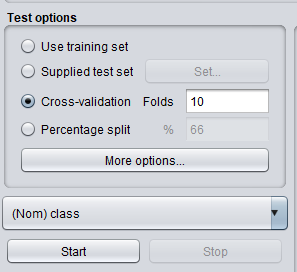
\includegraphics[width=0.60\linewidth]{imgs/capitolo4/weka_kcross.png}
     \caption{K-fold in weka}
     \label{fig:wekacross}
   \end{minipage}
\end{figure}

\section{Precision e Recall}
\label{par:precisionRecall}
Per valutare la bontà di una predizione da parte di un modello di machine learning si utilizzano varie metriche. Tra le più utilizzate troviamo al precision e la recall. Distinguiamo in un processo predittivo i falsi positivi, ovvero quelle istanze etichettate come appartenenti ad una classe ma che in realtà non lo sono ed i veri positivi, ovvero quelle istanze etichettate come appartenenti ad un classe e che lo sono realmente.
\begin{itemize}
    \item \textbf{Precision}: è data dal rapporto tra il numero di veri positivi ed il numero totale di elementi etichettati come appratenti ad una classe, dunque la somma di veri e falsi positivi. Un modello preciso genera pochi falsi positivi, perché quando prevede l'appartenenza ad una classe raramente sbaglia, mentre i falsi negativi potrebbero essere molti non prevedendo quindi tutte le istanze che dovrebbero appartenere ad una classe. Dunque la precision peggiora se vi sono tanti falsi positivi. 
    \item \textbf{Recall}: Questa metrica è data dal rapporto tra il numero di veri positivi ed il numero di istanze che realmente vi appartengono. Un alto valore di recall indica che il modello recupera tutte le istanze che appartengono alla classe. Tuttavia potrebbero esserci molti falsi positivi. Dunque la recall peggiora se vi sono tanti falsi negativi. 
\end{itemize}
Spesso accade che al migliorare della precisione si assiste ad un peggioramento della recall e viceversa. Bisogna dunque trovare un modello che cerchi un giusto compromesso. 